\chapter[Solar System]{Discovering and Characterizing Small Bodies in
  the Solar System}
\def\chpname{solarsystem}\label{chp:\chpname}

Chapter editors:
\credit{rhiannonlynne},
\credit{davidtrilling}.

Contributing authors:
\credit{ivezic},
\credit{migueldvb}.

% \section*{Summary}
% \addcontentsline{toc}{section}{~~~~~~~~~Summary}
%
% Executive summary goes here, highlighting the primary conclusions from
% the chapter's science cases. This should be abstract length, no more:
% say, 200 words.

% ====================================================================

\section{Introduction}
\label{sec:\chpname:intro}

LSST has tremendous potential as a discovery and characterization tool
for small bodies in the Solar System. With LSST, we have the
opportunity to increase our sample sizes of Potentially Hazardous
Asteroids (PHAs), Near Earth Objects (NEOs), Main Belt Asteroids
(MBAs), Jupiter Trojans, Centaurs, Trans-Neptunian Objects (TNOs),
Scattered Disk Objects (SDOs), comets and other small body populations
such as Earth mini-moons, irregular satellites, and other planetary
Trojan populations, by at least an order of
magnitude, often two orders of magnitude or more. In addition to
hundreds of astrometric measurements for most objects, LSST will also
provide precisely calibrated multiband photometry. With this
information, we can also characterize these populations -- deriving
colors, light curves, rotation periods, spin states, and even shape
models where possible.

The motivation behind studying these small body populations is
fundamentally to understand planet formation and evolution. The
orbital parameters of these populations record traces of the orbital
evolution of the giant planets. The migration of Jupiter, Saturn and
Neptune in particular have left marks on the orbital distribution of
MBAs, Jupiter Trojans, TNOs and SDOs. Rapid migration of
Jupiter and Saturn may have emplaced a large number of planetesimals
in the Scattered Disk; later slow migration of Neptune will affect the
number of TNOs in resonance and the details of their orbital parameters
within the resonance. Adding color information provides further
insights; colors roughly track composition, indicating formation
location and temperature or space weathering history. For example, the color
gradient of main belt asteroids, combined with their orbital
distribution, suggests that perhaps Jupiter migrated inwards,
mixing planetesimals from the outer Solar System into the outer parts
of the main belt, before eventually migrating outwards. Studying the
size distribution of each of the small body populations themselves
provides more constraints on planetesimal formation; this is
complicated by the effects of dynamical stirring from the giant
planets, which can increase the rate of erosion vs.\ growth during
collisions, and by the existence of the remnants of collisions such as
collisional families in the main belt. The presence of binaries and range
of spin states and shapes provides further constraints on the history
of each population. The location
of the planets before migration, the amount of migration, and the size
distribution of the small bodies themselves (after detangling the
dynamical evolution) all tell a deeper story about how the planets in
the Solar System formed, and how our formation history fits into the
range of observed extrasolar planetary systems.

These Solar System populations are unique when compared to other
objects which will be investigated by LSST, due to the simple fact
that they move across the sky. Metrics to evaluate
LSST's performance for moving objects need to be based on `per object'
measurements, rather than at a series of points on the sky or per
field pointing. For all metrics discussed in this chapter, the orbit
of each object is integrated over the time of the simulated opsim
survey and the detections of each object are recorded (using the
footprint of the focal plane and including
trailing losses and adjusting for the colors of the objects in each
filter to generate SNR and likelihood of detection); these
series of observations per object are then the basis for metric
evaluations.


% ====================================================================

% ====================================================================
%+
% SECTION:
%    SolarSystem_Discovery.tex
%
% CHAPTER:
%    solarsystem.tex
%
% ELEVATOR PITCH:
%    Discovery of solar system objects, all objects.
%    Figure of merit is completeness.
%
%-
% ====================================================================

\section{Discovery: Linking Solar System Objects}
\def\secname{\chpname:discovery}\label{sec:\secname}

\credit{rhiannonlynne},
\credit{davidtrilling},
\credit{ivezic}

Discovering, rather than simply detecting, small objects throughout
the Solar System requires unambiguously linking a series of detections
together into an orbit. The orbit provides the information necessary
to scientifically characterize the object itself and to understand the
population as a whole. Without orbits, the detections of Solar System
Objects (SSOs) by LSST will be of limited use; objects discovered with
other facilities could be followed up by LSST, but almost the entire
science benefit to planetary astronomy would be lost. Linking and
orbit determination for Solar System objects is similar to source
association for non-moving objects; it provides the means to identify
multiple detections as coming from a single object.

Therefore, the first concern regarding the Solar System is related
to the question ``Can we accurately link individual detections of moving objects into
orbits?''.  This requirement poses varying levels of difficulty as we
move from Near Earth Objects (NEOs) through the Main Belt Asteroids
(MBAs) and to Trans-Neptunian Objects (TNOs) and Scattered Disk Objects
(SDOs), as well as for comets and for other unusual but very
interesting populations such as Earth minimoons
(see Bolin et al.\ 2014).
Due to their small
heliocentric and geocentric distances, NEOs appear to move with
relatively high velocities and are distributed over a large fraction
of the sky, including regions far from the ecliptic plane. MBAs are densely distributed,
primarily within about 30 degrees of the ecliptic. TNOs and SDOs move
slowly, however short time intervals between repeat visits in each night may make these difficult
to link. Comets and Earth mini-moons may require more complicated
orbit fitting to allow for non-gravitational or geocentric
orbits. The requirements of accurately linking individual detections
into orbits also implies that we do not create false objects by
incorrectly linking detections and/or noise.

Much of the answer to this question comes down to the performance of
various pieces of LSST Data Management software. In particular,
important questions are the
rate of false positive detections resulting from difference imaging, possible
limitations of the Moving Object Processing System (MOPS) to extend to high
apparent velocities, and the capability to unambiguously determine if
a linkage is `real' or not via orbit determination (done as part of
MOPS). Thus this question includes concerns beyond the limits of the OpSim simulated
surveys, although it still bears on the observing strategy requirements for
discovering Solar System Objects. An in-depth study of the performance
of difference imaging and MOPS is currently ongoing. However, we can
make a range of assumptions on how MOPS will perform and evaluate how
many and which objects can be linked under observational cadence, given those assumptions.

It is important to emphasize that for the vast majority of
LSST-observed moving objects, LSST will be both the discovery and the
recovery facility. Most LSST-observed objects will be too faint
to be observed by assets that are currently carrying out
Solar System small bodies observations, and the number of 
detections will be so large that the existing infrastructure
could not observe more than a tiny fraction, even if they 
were bright enough. Therefore, as described in this section,
LSST's performance for detecting and re-detecting minor
bodies is critical to the success of the project; no outside
contributions will be significant.


% --------------------------------------------------------------------

\subsection{Target measurements and discoveries}
\label{sec:\secname:targets}

The criteria for `discovery' with MOPS depends on the number
of observations of an object acquired per night within some time
window (creating `tracklets'), repeated over a number of nights within window of some
days (creating `tracks'), which are then linked into an orbit with a threshold on
astrometric residuals. The current assumptions are that we can link
detections into orbits with 2 detections per night within 90 minutes,
repeated for 3 nights within a window of 15 days. The additional assumptions are
that with these 6 observations, we will be able to create low-accuracy orbits that will suffice to link
additional observations obtained at later (or earlier, in the LSST
archive) times, and that the orbit fitting will enable rejection
of mislinkages.

We can also use other requirements for discovery. Requiring 4
detections in each night is a fairly common discovery criteria for
NEO surveys, as it reduces the number of mislinked tracklets to almost
zero. We could also require 4 nights of pairs within a window of 20 days, in order to improve the
initial orbit fitting and mislinkage rejection. We can also assume
MOPS will perform better than the current assumptions, and evaluate
discovery criteria of 3 pairs within a 30 day window.

With these discovery criteria, we can then evaluate the completeness
of an LSST simulated survey, for a given population. We can look at
this as a function of H magnitude and as a function of orbital
parameters.

For PHAs and NEOs there are special considerations in terms of
completion that arise from planetary defense concerns. For most other
populations, the general desire is simply to have a high level of
completeness, with no gaps in completeness that depend strongly on
orbital parameters. In particular, the desire is to be able to
calibrate any selection effects in discovery so that the survey completeness can
be used to debias the underlying population models.

Discovery opportunity, and thus the completeness of the underlying
population, is very sensitive to the time interval between
observations. Waiting longer between observations within a night means that objects
may move beyond a single LSST field of view. Longer times between
revisits means that observing in large contiguous blocks (rather than
narrow, disconnected strips) within a night becomes more important to make sure that
objects are followed between pointings, especially if the time
interval is much longer than 30 minutes. Because the objects must be
detected on several nights within the window, the inter-night revisit
rate for similar large contiguous blocks of sky is important.

An optimal discovery strategy for moving
objects could be ensuring a minimum (default: two) number of revisits
within a night within a short time window (default: 90 minutes),
preferably over a large block of sky, and
covering large contiguous amounts of sky several (default: 3) times within a
longer time window (default: 15 days).  Observations within a single
night do not need to be in the same filter, however we will be
constrained by the shallower limiting magnitude of the pair; {\it e.g.}
preferably $r$ band observations would be paired with $i$ rather than
$u$ observations. Finally, the fill factor of the camera is important;
in these simulations we have used the LSST focal plane, which has an
approximately 92\% fill factor.

% --------------------------------------------------------------------

\subsection{Metrics}
\label{sec:\secname:metrics}

The {\tt DiscoveryChancesMetric} can be used to identify sets of
detections of a particular object that meet the defined criteria for
discovery: X detections within T minutes in a night, Y nights within a
W day window; this describes the number of discovery opportunities for
each object. The results from the Discovery Metric can be fed to the
{\tt MoCompletenessMetric} summary metric, where if an object achieves
a user-defined requirement for the minimum number of discovery
opportunities (typically 1), then it is counted as `discovered'.  The
total number of objects discovered at each H magnitude is compared to
the total number of objects in the population at that H magnitude, in
order to evaluate `completeness' as a function of H. Discovery
opportunities can be evaluated as a function of orbital parameters, to
look for areas of orbital space that may be missed in a particular
survey strategy; completeness, since it marginalizes over the entire
population at a particular H value, loses this
capability. Completeness can be evaluated as a differential value
(completeness @ H=X) or integrated over the size distribution
(completeness @ H $\leq$ X).

The completeness can be parametrized by the completeness ($C_b$) at
some bright absolute magnitude ($H_b$), combined with the magnitude at
which this falls to 50\% ($H_f$). A draft set of requirements for
these parameters has been written up in the Solar System Object
Specifications document, although these requirements are still quite
preliminary. The current goal parameters are described in Table~\ref{ssoreqs}.

\begin{table}[]
\centering
\caption{Solar System Object Differential Completeness Goals}
\label{ssoreqs}
\begin{tabular}{llll}
    & $C_b$ & $H_b$ & $H_f$ \\
NEA & 80\%  & 18.4  & 21.9  \\
MBA & 90\%  & 19.5  & 20.2  \\
TNO & 90\%  & 7.0   & 8.1
\end{tabular}
\end{table}

A further simplification of the completeness can be achieved by simply
measuring the completeness at a preset absolute magnitude. For
example, completeness for PHAs at H=22 is an important summary value,
and is discussed in its own section, \ref{sec:solarsystem:phas}.


% --------------------------------------------------------------------

\subsection{OpSim Analysis}
\label{sec:\secname:analysis}

The basic output from the {\tt DiscoveryChancesMetric} is the number
of discovery opportunities (e.g.\ sets of observations that match the
required discovery criteria) available. For objects which have at
least a given number of discovery opportunities (here, we simply use
one required opportunity), then this object can be considered
``found'' and marked towards the completeness of the population at a
given H magnitude with the {\tt MoCompletenessMetric} summary metric.
Examining the \opsimdbref{db:baseCadence} Baseline Cadence with these metrics,
we find that most objects have many discovery opportunities. This is shown in
Figure~\ref{standard_discovery}.

\begin{figure}
\includegraphics[width=3.3in]{figs/solarsystem/minion_1016_DiscoveryChances_tno_mba_neo_10_year_3_pairs_in_15_nights_MOOB_ComboMetricVsH}
\includegraphics[width=3.3in]{figs/solarsystem/minion_1016_CumulativeCompleteness_tno_mba_neo_10_year_3_pairs_in_15_nights_MOOB_ComboMetricVsH}
\caption{Left: Number of discovery chances as a function of H
  (mean value for all objects at each $H$ value), assuming the minimum criteria for
  discovery - 2 visits per night within 90 minutes, repeated for 3
  nights within 15 days. Right: Resulting cumulative completeness for
  each population, assuming that only 1 discovery opportunity is
  required to `discover' each object.
\label{standard_discovery}}
\end{figure}

The runs \opsimdbref{db:baseCadence}, \opsimdbref{db:NoVisitPairs},
\opsimdbref{db:NEOswithVisitTriplets}, \opsimdbref{db:NEOwithVisitQuads}
are particularly interesting to evaluate in light of the different
sets of discovery criteria. Because OpSim does not currently require
only pairs (or singles, triplets or quads), but instead will sometimes
acquire more than the requested number of visits, changing the
discovery criteria from pairs within a night to triplets or quads,
does not automatically cause the completeness to plummet, although it
does decrease. Looking at the raw numbers of discovery chances offers some
enlightenment: the number of discovery opportunities does falls dramatically as we go from pairs to quads, however, there
are still some times when observations are obtained in triplets or
quads, so there are still some discovery chances. This behavior of the
scheduler (to frequently acquire more than the requested number of
visits) is likely to change in the future and make this effect more pronounced, but the completeness will
clearly be very sensitive to how observations are acquired. This effect is shown in
Figure~\ref{completeness_changes}.

\begin{figure}
\includegraphics[width=3.3in]{figs/solarsystem/minion_1016_CumulativeCompleteness_pairs_20_4_quads_3_30_3_30_triplets_3_30_pairs_3_15_pairs_nights_in_neo_year_10_MOOB_ComboMetricVsH}
\includegraphics[width=3.3in]{figs/solarsystem/kraken_1043_CumulativeCompleteness_pairs_20_4_quads_3_30_3_30_triplets_3_30_pairs_3_15_pairs_nights_in_neo_year_10_MOOB_ComboMetricVsH} \\
\includegraphics[width=3.3in]{figs/solarsystem/enigma_1281_CumulativeCompleteness_pairs_20_4_quads_3_30_3_30_triplets_3_30_pairs_3_15_pairs_nights_in_neo_year_10_MOOB_ComboMetricVsH}
\includegraphics[width=3.3in]{figs/solarsystem/enigma_1282_CumulativeCompleteness_pairs_20_4_quads_3_30_3_30_triplets_3_30_pairs_3_15_pairs_nights_in_neo_year_10_MOOB_ComboMetricVsH}
\caption{Cumulative completeness for an NEO population, given
  different sets of discovery criteria, for the \opsimdbref{db:baseCadence}, \opsimdbref{db:NoVisitPairs},
\opsimdbref{db:NEOswithVisitTriplets},
\opsimdbref{db:NEOwithVisitQuads} simulated surveys. The results in the
lower right come from a simulated survey, \opsimdbref{db:NEOwithVisitQuads},
which attempted to obtain four visits to each field in each
night; the results on the upper left, come from the baseline simulated
survey, \opsimdbref{db:baseCadence}, which attempts to obtain pairs of
visits.
\label{completeness_changes}}
\end{figure}

Another aspect to consider is to look at how the completeness
increases over time. The completeness as a function of time is plotted
for particular $H$ values, depending on the
population, in Figure~\ref{completeness_time}.

\begin{figure}
\includegraphics[width=2in]{figs/solarsystem/minion_1016_neo_CompletenessOverTime_22_time}
\includegraphics[width=2in]{figs/solarsystem/minion_1016_mba_CompletenessOverTime_20_time}
\includegraphics[width=2in]{figs/solarsystem/minion_1016_tno_CompletenessOverTime_8_time}
\caption{Completeness as a function of time, for NEO, MBA and TNO
  populations. The completeness increases rapidly for the first few
  years, then increases more slowly. The NEO completeness rises more
  slowly than other populations, as more NEOs become available to
  discover due to changing their orbital positioning relative to Earth
  (becoming closer and brighter, or moving away from sightlines behind
  the Sun). The TNO completeness rises most rapidly with time, as
  these objects move slowly; we find most of these objects within the
  first two years and then improve their characterization over the
  rest of the survey (measuring better orbits and obtaining
  lightcurves and colors).
\label{completeness_time}}
\end{figure}

\begin{table}[]
\centering
\caption{Solar System Object Differential Completeness in \opsimdbref{db:baseCadence}}
\label{ssoperf}
\begin{tabular}{llll}
    & $C_b$ & $H_b$ & $H_f$ \\
NEA & 87.5\%  & 18.5  & 21.5  \\
MBA & 89\%  & 19.5  & 20.2  \\
TNO & 96\%  & 7.0   & 8.3
\end{tabular}
\end{table}



% --------------------------------------------------------------------

\subsection{Discussion}
\label{sec:\secname:discussion}

A large portion of the risk in being able to discover moving objects
lies in the currently uncertain performance of the MOPS
software. Figure~\ref{completeness_changes} clearly shows that with
the baseline cadence, if we must have triplets or pairs, or even just
require 4 pairs of observations over 20 nights, that the completeness
falls. The performance will likely fall even further if the scheduler
stops obtaining more than the minimum requested number of observations.

With the expected MOPS discovery requirements,
\opsimdbref{db:baseCadence} performs adequately for most solar system
objects, although completeness falls off more rapidly for faint
objects than desired for NEOs. To investigate this effect, more
metrics will have to be developed to discover why these fainter NEOs
are not being discovered (are they simply missing appropriate
sequences of observations due to the cadence or is something more
subtle occurring?).

% ====================================================================
%
% \subsection{Conclusions}
%
% Here we answer the ten questions posed in
% \autoref{sec:intro:evaluation:caseConclusions}:
%
% \begin{description}
%
% \item[Q1:] {\it Does the science case place any constraints on the
% tradeoff between the sky coverage and coadded depth? For example, should
% the sky coverage be maximized (to $\sim$30,000 deg$^2$, as e.g., in
% Pan-STARRS) or the number of detected galaxies (the current baseline but
% with 18,000 deg$^2$)?}
%
% \item[A1:] ...
%
% \item[Q2:] {\it Does the science case place any constraints on the
% tradeoff between uniformity of sampling and frequency of  sampling? For
% example, a rolling cadence can provide enhanced sample rates over a part
% of the survey or the entire survey for a designated time at the cost of
% reduced sample rate the rest of the time (while maintaining the nominal
% total visit counts).}
%
% \item[A2:] ...
%
% \item[Q3:] {\it Does the science case place any constraints on the
% tradeoff between the single-visit depth and the number of visits
% (especially in the $u$-band where longer exposures would minimize the
% impact of the readout noise)?}
%
% \item[A3:] ...
%
% \item[Q4:] {\it Does the science case place any constraints on the
% Galactic plane coverage (spatial coverage, temporal sampling, visits per
% band)?}
%
% \item[A4:] ...
%
% \item[Q5:] {\it Does the science case place any constraints on the
% fraction of observing time allocated to each band?}
%
% \item[A5:] ...
%
% \item[Q6:] {\it Does the science case place any constraints on the
% cadence for deep drilling fields?}
%
% \item[A6:] ...
%
% \item[Q7:] {\it Assuming two visits per night, would the science case
% benefit if they are obtained in the same band or not?}
%
% \item[A7:] ...
%
% \item[Q8:] {\it Will the case science benefit from a special cadence
% prescription during commissioning or early in the survey, such as:
% acquiring a full 10-year count of visits for a small area (either in all
% the bands or in a  selected set); a greatly enhanced cadence for a small
% area?}
%
% \item[A8:] ...
%
% \item[Q9:] {\it Does the science case place any constraints on the
% sampling of observing conditions (e.g., seeing, dark sky, airmass),
% possibly as a function of band, etc.?}
%
% \item[A9:] ...
%
% \item[Q10:] {\it Does the case have science drivers that would require
% real-time exposure time optimization to obtain nearly constant
% single-visit limiting depth?}
%
% \item[A10:] ...
%
% \end{description}

\navigationbar


% ====================================================================

% ====================================================================
%+
% SECTION:
%    SolarSystem_PHA.tex
%
% CHAPTER:
%    solarsystem.tex
%
% ELEVATOR PITCH:
%    Discovery of PHAs in particular. Discussion of wider 'impacts'.
%
%-
% ====================================================================

\section{Discovery of Potentially Hazardous Asteroids}
\def\secname{\chpname:phas}\label{sec:\secname}

\credit{ivezic},
\credit{rhiannonlynne}.

The U.S. Congress has given a mandate to NASA to implement a
Near-Earth Object (NEO) Survey program to detect, track, catalog, and
characterize the physical characteristics of near-Earth objects equal
to or greater than 140 meters in diameter\footnote{See
\url{http://www.gpo.gov/fdsys/pkg/PLAW-109publ155/pdf/PLAW-109publ155.pdf}}. The
goal is to achieve a completeness of 90\%. In recent practice, adopted
here, the completeness is evaluated for a subset of NEOs called
Potentially Hazardous Asteroids\footnote{Potentially Hazardous
Asteroids (PHAs) are defined as asteroids with a minimum orbit
intersection distance (MOID) of 0.05 AU or less.} (PHA), with
H$\le$22, where H is the absolute magnitude\footnote{Absolute
magnitude is the magnitude that an asteroid would have at a distance
of 1 AU from the Sun and from the Earth, viewed at zero phase
angle. This is an impossible configuration, of course, but the
definition is motivated by desire to separate asteroid physical
characteristics from the observing configuration.} in the Johnson's V
band.

The discovery criteria for PHAs follows the same guidelines and metrics found in the previous
section, \ref{sec:solarsystem:discovery}, but is worth discussing
separately to focus on its main figure
of merit - completeness for PHAs with H$\le$22 magnitudes.

% --------------------------------------------------------------------

\subsection{Target measurements and discoveries}
\label{sec:\secname:targets}

Using the same range of discovery criteria as in the previous section,
\ref{sec:solarsystem:discovery}, we can look at the differential and
cumulative completeness for a population of PHAs. For this sample of
PHAs, we pulled the orbits of 2,000 objects with MOID~$<= 0.05$~AU from 
the Grav S3M model \citep{2011PASP..123..423G}. These orbits were
then cloned over a range of $H$ values to evaluate the chances of
discovery for that orbit at each of those $H$ values. The differential
completeness as a function of $H$ is then simply the fraction of
objects which receive at least one set of observations which meet the
discovery criteria during the course of the survey. The cumulative
completeness is similar, but integrated over $H$ by assuming an $H$
distribution with a power-law index of $\alpha=0.3$. Both
differential and cumulative completeness are relevant metrics: the
former provides more insight in the behavior of a particular
simulation, while the latter is a metric given to NASA by the U.S.
Congress.

To match the NEO mandate, the cumulative completeness at $H$=22 can be
used as a figure of merit.

% --------------------------------------------------------------------

\subsection{Metrics}
\label{sec:\secname:metrics}

The metrics used here are the same as in
\ref{sec:solarsystem:discovery}, although run with different input populations.

% --------------------------------------------------------------------

\subsection{OpSim Analysis}
\label{sec:\secname:analysis}

The differential and cumulative completeness for the baseline survey,
\opsimdbref{db:baseCadence}, at a range of years is shown in
\autoref{fig:baselinePHA}. The baseline cadence achieves a cumulative completeness of 66\% for
H$\le$22 PHAs when requiring pairs of visits on 3 separate nights within 15 days. 
The differential completeness at $H$=22 for the same
survey is 49\%, 17\% lower due to increasing completeness toward
smaller $H$ (larger objects).

%%%%%%%%%%%%%%%%%%%%%%%%%%%
\begin{figure}[th]
%\vskip -1.1in
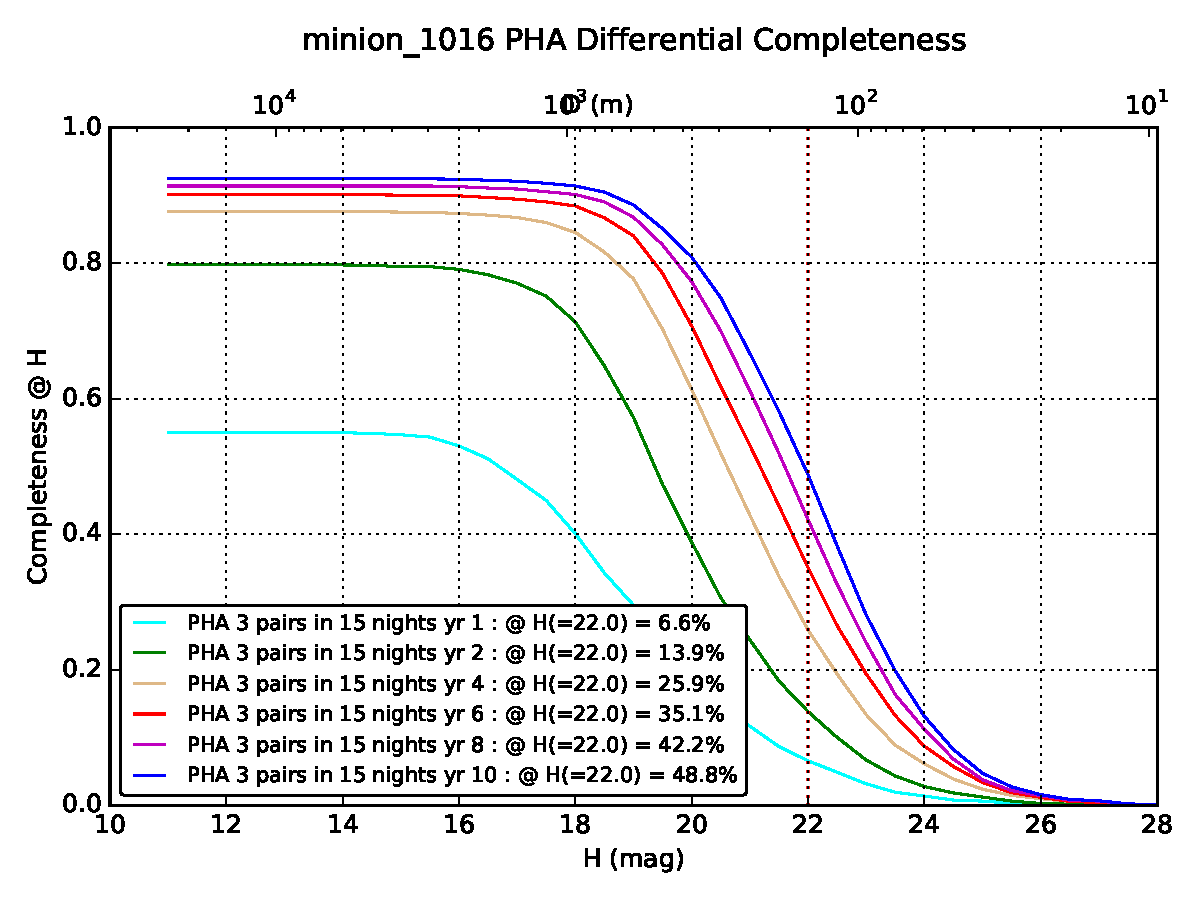
\includegraphics[angle=0,width=0.49\hsize:,clip]{figs/solarsystem/minion_1016_DifferentialCompleteness_PHA_3_pairs_in_15_nights_Years_1_to_10_MOOB_ComboMetricVsH}
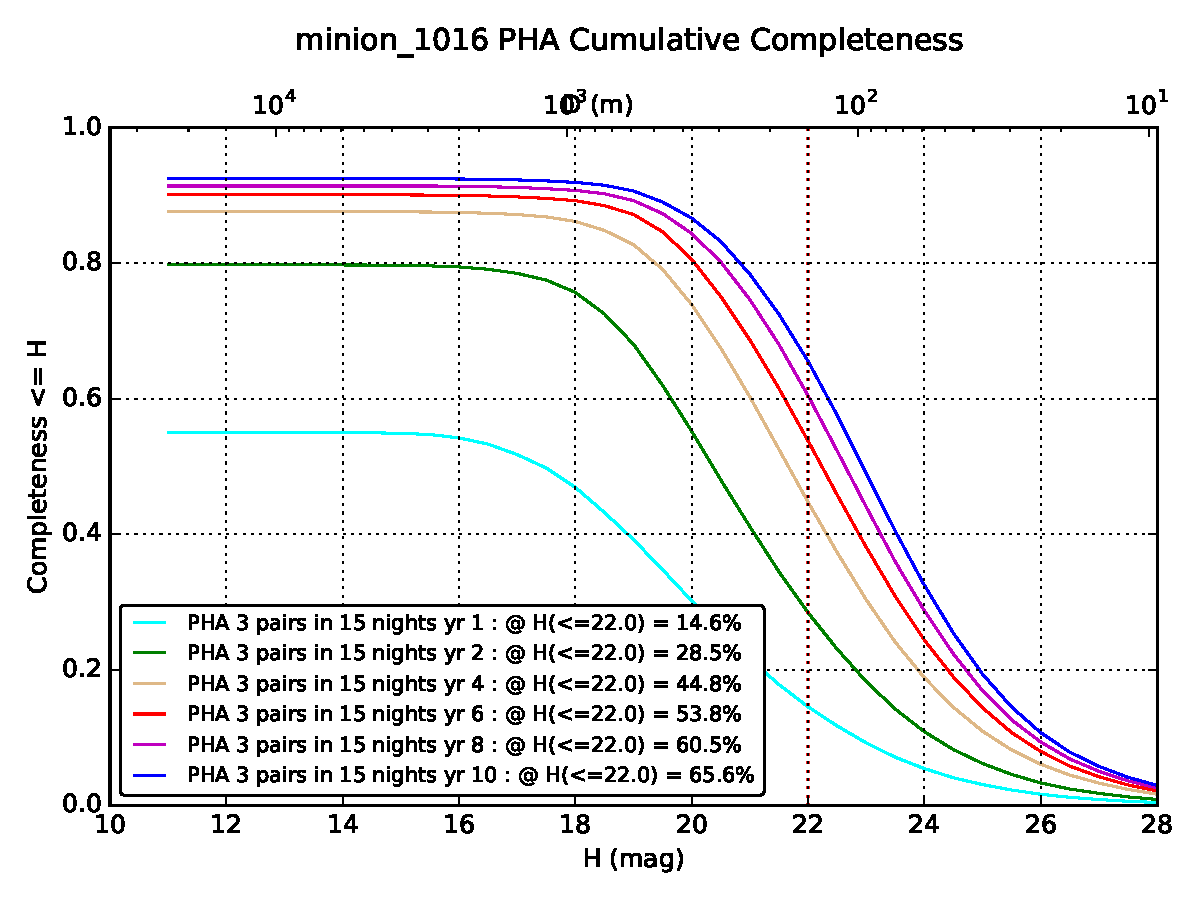
\includegraphics[angle=0,width=0.49\hsize:,clip]{figs/solarsystem/minion_1016_CumulativeCompleteness_PHA_3_pairs_in_15_nights_Years_1_to_10_MOOB_ComboMetricVsH}
%\vskip -1.2in
\caption{The PHA completeness for \opsimdbref{db:baseCadence}, as a function of the object's absolute
visual magnitude H on the horizontal axes (left: differential completeness at a given H;
right: cumulative completeness for all objects brighter than a given H), as it increases year over year.
The cumulative completeness for H$\le$22 NEOs (those with diameters larger than 140m)  for this
simulation is 66\% after 10 years.}
\label{fig:baselinePHA}
\end{figure}
%%%%%%%%%%%%%%%%%%%%%%%%%%%

We find that the PHA and NEO completeness are very similar for a given simulated survey and set of discovery criteria, as shown in \autoref{fig:neopha},
a reasonable result given that the input populations are very similar.
The analysis of the various observing run strategies (singles, pairs, triples or quads of visits) described in the previous section thus applies to PHAs as well.

%%%%%%%%%%%%%%%%%%%%%%%%%%%
\begin{figure}[bh]
%\vskip -1.2in
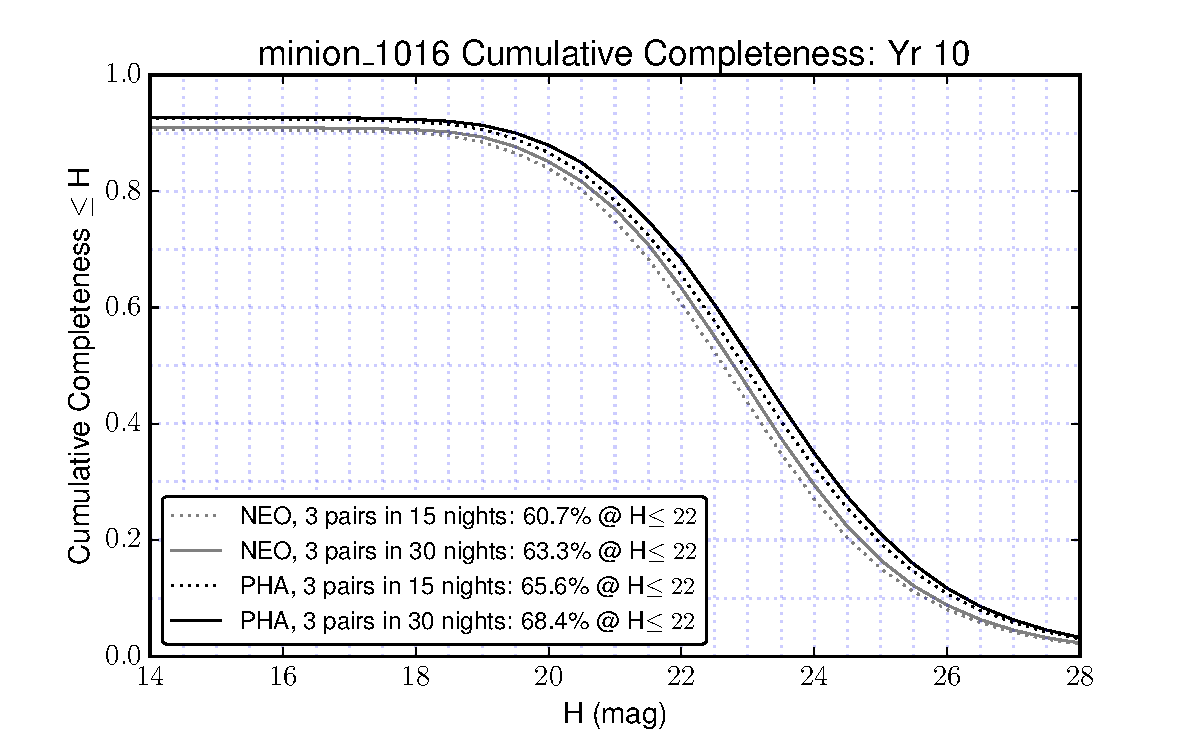
\includegraphics[angle=0,width=0.49\hsize:,clip]{figs/solarsystem/minion_1016_CumulativeCompleteness_NEO_and_PHA_Cumulative_Completeness}
%\vskip -1.3in
\caption{%
Comparison of the cumulative NEO and PHA completeness for the baseline cadence
\opsimdbref{db:baseCadence}.}
\label{fig:neopha}
\end{figure}
%%%%%%%%%%%%%%%%%%%%%%%%%%%

% ====================================================================
%
% \subsection{Conclusions}
%
% Here we answer the ten questions posed in
% \autoref{sec:intro:evaluation:caseConclusions}:
%
% \begin{description}
%
% \item[Q1:] {\it Does the science case place any constraints on the
% tradeoff between the sky coverage and coadded depth? For example, should
% the sky coverage be maximized (to $\sim$30,000 deg$^2$, as e.g., in
% Pan-STARRS) or the number of detected galaxies (the current baseline 
% of 18,000 deg$^2$)?}
%
% \item[A1:] ...
%
% \item[Q2:] {\it Does the science case place any constraints on the
% tradeoff between uniformity of sampling and frequency of  sampling? For
% example, a rolling cadence can provide enhanced sample rates over a part
% of the survey or the entire survey for a designated time at the cost of
% reduced sample rate the rest of the time (while maintaining the nominal
% total visit counts).}
%
% \item[A2:] ...
%
% \item[Q3:] {\it Does the science case place any constraints on the
% tradeoff between the single-visit depth and the number of visits
% (especially in the $u$-band where longer exposures would minimize the
% impact of the readout noise)?}
%
% \item[A3:] ...
%
% \item[Q4:] {\it Does the science case place any constraints on the
% Galactic plane coverage (spatial coverage, temporal sampling, visits per
% band)?}
%
% \item[A4:] ...
%
% \item[Q5:] {\it Does the science case place any constraints on the
% fraction of observing time allocated to each band?}
%
% \item[A5:] ...
%
% \item[Q6:] {\it Does the science case place any constraints on the
% cadence for deep drilling fields?}
%
% \item[A6:] ...
%
% \item[Q7:] {\it Assuming two visits per night, would the science case
% benefit if they are obtained in the same band or not?}
%
% \item[A7:] ...
%
% \item[Q8:] {\it Will the case science benefit from a special cadence
% prescription during commissioning or early in the survey, such as:
% acquiring a full 10-year count of visits for a small area (either in all
% the bands or in a  selected set); a greatly enhanced cadence for a small
% area?}
%
% \item[A8:] ...
%
% \item[Q9:] {\it Does the science case place any constraints on the
% sampling of observing conditions (e.g., seeing, dark sky, airmass),
% possibly as a function of band, etc.?}
%
% \item[A9:] ...
%
% \item[Q10:] {\it Does the case have science drivers that would require
% real-time exposure time optimization to obtain nearly constant
% single-visit limiting depth?}
%
% \item[A10:] ...
%
% \end{description}

\navigationbar


% ====================================================================

% ====================================================================
%+
% SECTION:
%    SolarSystem_OrbitalAccuracy.tex
%
% CHAPTER:
%    solarsystem.tex
%
% ELEVATOR PITCH:
%    How secure is the orbit - is it going to hit us?
%    Libration amplitude distribution for TNOs?
%    Can we find it after X years for further study?
%    Can we identify the source region for NEOs within the main belt?
%-
% ====================================================================

\section{Orbital Accuracy}
\def\secname{\chpname:orbits}\label{sec:\secname}

\credit{rhiannonlynne},
\credit{davidtrilling}

A vast number of moving objects will appear in LSST images. Multiple
observations of a common object will be linked, and a preliminary orbit
derived. However, the orbital elements (semi-major axis, eccentricity,
etc.) will have some uncertainty. Short arcs --- that is, a small amount
of time between the first and last observation of a given object ---
produce orbits with large uncertainties on the orbital elements. As arc
length grows, the orbital uncertainties decrease.

A number of science cases require relatively small uncertainties on
orbital elements. Perhaps most importantly, small uncertainties can aid
in discriminating between Near Earth Objects that might and might not
impact the Earth. A more subtle example relates to the libration
amplitude distribution for TNOs, which can be compared to predictions
from Solar System formation models. Only with small uncertainties on
orbital elements can the libration amplitudes be determined to
sufficient precision to compare to the predictive models. Finally,
during and after the primary LSST survey additional measurements will be
desired for further characterization of many objects. Only if the
orbital elements are sufficiently well known can objects be studied later
with other facilities. For example, to carry out spectroscopy, the
position of the object must be known to approximately 1~arcsec (the
width of a typical slit). This places strong requirements on the
knowledge of the orbital elements.


% --------------------------------------------------------------------

\subsection{Target measurements and discoveries}
\label{sec:\secname:targets}

The relevant data here are positions as a function of time for a given
object (assuming that the linking of measurements to a given object is
satisfactory). Assuming that the accuracy and precision of each
measurement are approximately constant (likely, since all will be made
by the same observing system), the only significant factor that improves
the knowledge of the orbit is extending the observational arc. The
observing strategy employed by LSST must therefore have a cadence in
which objects are revisited with the largest possible arcs that still
allow linking of observations. In other words, if the observations of a
given object are too widely spaced, linking may not be possible, so,
even though the arc is long, the linking is poor and the object yield is
low. If the observations are made too densely in time, linking is likely
to be good, but the arc may not be very long. A middle ground is
desired.

% --------------------------------------------------------------------

\subsection{Metrics}
\label{sec:\secname:metrics}

The best metric here would be to take the actual series of observations
of each object, add appropriate astrometric noise to each observation
according to its SNR, cull observations which would not be `linkable' to
the rest (i.e.\ observations which occur on a single night far from other
nights in the arc, or even a series of observations which occur too many
years away from other observations of the same object), and then fit an
orbit to the remaining observations and determine the uncertainty in its
parameters. This is work for the future however; our first simple proxy
uses the \MAFmetric{ObsArcMetric} to just look at the time between the first
and last observation of an object. For many objects, this will be fairly
close to the actual arc length of the linkable observations, as most
objects receive many observations clumped together when they are
observable, so this simple proxy makes a reasonable starting point.


% --------------------------------------------------------------------

\subsection{OpSim Analysis}
\label{sec:\secname:analysis}

\begin{figure}
\includegraphics[width=6in]{figs/solarsystem/minion_1016_ObsArc_neo_tno_mba_MOOB_ComboMetricVsH}
\caption{Mean observational arc length, in years, for NEO, MBA and TNO
  populations as a function of $H$ magnitude.
\label{obsarc}}
\end{figure}

In \opsimdbref{db:baseCadence}, the mean observational arc length for
NEOs and MBAs is about 8~years for bodies larger than 1~km, and about
6~years for 300~m bodies. With these
orbital arcs, the orbits will be quite well known,
% xxx quantify -- how well! xxx,
meaning that the majority
of LSST-observed objects will have orbits that are sufficiently
well known that the above science cases can be carried out.
In some special cases --- for example, the case where
an NEO's orbit still presents a significant probability
of terrestrial impact --- additional non-LSST follow-up
may be needed, but this will be a small minority of cases.

% xxx what we probably want is fraction of objects
% with arcs longer than 3 years (say) as a fxn of
% H mag, for NEOs/MBAs/TNOs. xxx

% --------------------------------------------------------------------

\subsection{Discussion}
\label{sec:\secname:discussion}

The simple proxy metric above should be improved to account for
potential difficulties in linking observations, and to include actual
orbital fitting to determine orbital uncertainties. The timing of
observations effects the final orbital accuracy significantly,
particularly for TNOs, and having a good distribution on the times of
observations can improve orbital accuracy more quickly than would
naively be expected from a simple observational arclength scaling.

A figure of merit, including requirements on the orbital accuracy for
various classes of objects, should also be developed.

As an intermediate step, we have carried out two anecdotal studies
of orbital accuracy. In the first,
we took an arbitrary (real) NEO --- object 2016~DL ---
with a six year arc. This is representative
and typical of NEOs that will be observed
by LSST.
The maximum positional uncertainty for this object
over the next ten years
is 25~arcsec (3$\sigma$). This is small enough
that essentially any kind of follow-up observation would be
possible (presuming that pre-imaging is possible
for spectroscopy, for example, to locate the moving
object).
The uncertainties on the orbital parameters
of this object are on the order of
1 part in 10$^4$ or even smaller. This level of
precision should allow all the investigations described
above.

In the second experiment, we took an arbitrary
(real) TNO --- object 2015~SO20 ---
that has a five year arc.
For this object, the maximum positional uncertainty
over the next ten years is $\sim$20'', and its orbital
elements are known to
around 1 part in 10$^5$. Again, this level
of precision should enable all of the science
investigations described above.


% ====================================================================
%
% \subsection{Conclusions}
%
% Here we answer the ten questions posed in
% \autoref{sec:intro:evaluation:caseConclusions}:
%
% \begin{description}
%
% \item[Q1:] {\it Does the science case place any constraints on the
% tradeoff between the sky coverage and coadded depth? For example, should
% the sky coverage be maximized (to $\sim$30,000 deg$^2$, as e.g., in
% Pan-STARRS) or the number of detected galaxies (the current baseline
% of 18,000 deg$^2$)?}
%
% \item[A1:] ...
%
% \item[Q2:] {\it Does the science case place any constraints on the
% tradeoff between uniformity of sampling and frequency of  sampling? For
% example, a rolling cadence can provide enhanced sample rates over a part
% of the survey or the entire survey for a designated time at the cost of
% reduced sample rate the rest of the time (while maintaining the nominal
% total visit counts).}
%
% \item[A2:] ...
%
% \item[Q3:] {\it Does the science case place any constraints on the
% tradeoff between the single-visit depth and the number of visits
% (especially in the $u$-band where longer exposures would minimize the
% impact of the readout noise)?}
%
% \item[A3:] ...
%
% \item[Q4:] {\it Does the science case place any constraints on the
% Galactic plane coverage (spatial coverage, temporal sampling, visits per
% band)?}
%
% \item[A4:] ...
%
% \item[Q5:] {\it Does the science case place any constraints on the
% fraction of observing time allocated to each band?}
%
% \item[A5:] ...
%
% \item[Q6:] {\it Does the science case place any constraints on the
% cadence for deep drilling fields?}
%
% \item[A6:] ...
%
% \item[Q7:] {\it Assuming two visits per night, would the science case
% benefit if they are obtained in the same band or not?}
%
% \item[A7:] ...
%
% \item[Q8:] {\it Will the case science benefit from a special cadence
% prescription during commissioning or early in the survey, such as:
% acquiring a full 10-year count of visits for a small area (either in all
% the bands or in a  selected set); a greatly enhanced cadence for a small
% area?}
%
% \item[A8:] ...
%
% \item[Q9:] {\it Does the science case place any constraints on the
% sampling of observing conditions (e.g., seeing, dark sky, airmass),
% possibly as a function of band, etc.?}
%
% \item[A9:] ...
%
% \item[Q10:] {\it Does the case have science drivers that would require
% real-time exposure time optimization to obtain nearly constant
% single-visit limiting depth?}
%
% \item[A10:] ...
%
% \end{description}

% --------------------------------------------------------------------

\navigationbar


% ====================================================================

% ====================================================================
%+
% SECTION:
%    SolarSystem_CometActivity.tex
%
% CHAPTER:
%    solarsystem.tex
%
% ELEVATOR PITCH:
%-
% ====================================================================

\section{Detecting Comet Activity}
\def\secname{\chpname:activity}\label{sec:\secname}

\credit{rhiannonlynne},
\credit{davidtrilling},
\credit{migueldvb}

Comets are the remnant building blocks of the Solar System
that have been stored at cold temperatures beyond the ice
line, either in the Kuiper belt or the Oort cloud, since their
formation.  Measuring the evolution of cometary activity over
a range of heliocentric distances with LSST will allow us to
understand the overall comet activity and to link these
observations with the physical and chemical conditions in the
early solar nebula during planet formation.  Comets are
classified in two main dynamical families, Jupiter Family
comets (JFCs) that have low-inclination orbits with periods
less than 20 years, and Long-period comets (LPCs) that
originate in the Oort Cloud at a distance of more than 10000
AU and have large orbital eccentricities and nearly isotropic
distribution of inclinations.  Currently there are over 400
Jupiter-family comets known, most of which are faint compared
with the LPCs.  LSST will observe about $10^4$ individual
comets repeatedly including measurements of known objects over
its 10-year survey \citep{2010PhDT.......241S}. The
determination of their activity levels at various heliocentric
distances will be used to study the time evolution of each
object individually and to find the connection between comet
families and their formation region in the Solar System.

Several cometary volatiles result in strong emission bands
excited by solar radiation that emit by resonant fluorescence
at optical and near-ultraviolet wavelengths.  The LSST $u$
filter peaks near the CN (0--0) emission band at 3880 \r{A}.
Although CN is not the most abundant daughter species from
cometary volatiles and the OH (0--0) emission band at 3080
\r{A} is generally stronger, CN production rates provide an
excellent proxy of the level of overall gas activity in
comets. LSST will offer a unique opportunity to produce
a large database of CN production rates, vastly increasing our current
knowledge \citep[see
e.g.][]{1995Icar..118..223A, 2012ApJ...758...29A}.
 Other bands such as $r$, $i$, and $z$ will detect
continuum brightness that is produced by reflected radiation
from dust particles in the coma. Thus, it will be possible to
obtain the evolution of the gas-to-dust production ratio at
high cadence as a function of heliocentric distance in
different comet families. The greatly increased sample size
compared with previous catalogs \citep{1995Icar..118..223A}
will allow for statistical comparison of the comet families
and to link them to other small body populations in the Solar
System.

A recently discovered population of main-belt asteroids eject
dust and produce coma and tails giving them the appearance of
comets \citep{2012AJ....143...66J}.  This so-called main-belt
comets or active asteroids have the orbital characteristics of
asteroids with $T_J > 3$ and lose mass during part of their
orbits. The cometary activity observed in these objects may be
driven by primordial water water ice that is trapped near the
surface and sublimates when it is exposed to sunlight.
Main-belt comets are important because they may have been able to
preserve water ice despite the effect of solar radiation and
heating from the decay of short-lived radioactive nuclei.  The
asteroids in the outer regions of the main belt can therefore
have a substantial fraction of water and other volatiles that
may have supplied the volatile content of terrestrial planets.
Most of the main-belt-comets are faint with very weak comae
that are active during part of their orbits. Given the
expected flux sensitivity of LSST, the transient cometary
activity of main-belt asteroids will be observable including
many objects that could be below the detection limits of
current photometric surveys.  The LSST observations will thus
help to understand the overlap between different populations
in the Solar System such as the relationship between comets
and asteroids.

% --------------------------------------------------------------------

\subsection{Target measurements and discoveries}
\label{sec:\secname:targets}

LSST will make an exceptionally large number of comet
observations.  About $10^4$ comets will be observed on average
of 50 times by LSST during its main survey, while a few objects
will be observed more than 1000 times
\citep{2010PhDT.......241S}.  Simulations of characteristic
comet orbits have shown that LSST will observe some Jupiter
Family comets (JFCs) hundreds of times over their full orbits
\citep{2010PhDT.......241S}.  Individual LPCs are predicted to
be observed by LSST with dozens of observations as they
approach or recede from the center of the Solar System or
during their perihelion passage.  Thus, these observations
will trace the onset of outgassing from quiescence at large
heliocentric distances and the decline of activity after
perihelion.

Ensuring that any activity or outgassing of a comet or active asteroid
is clearly identifiable with LSST DM or contributed Level 3 software is not a
solved problem, however there is ongoing work toward this goal (xx
ref? Hsieh, other? xx). In the meantime, it does not seem unreasonable
to assume that the main requirement, in terms of cadence, is to actually
have an observation at a time when activity is visible, as well as at
surrounding times to determine the start and end points of that activity.

Cometary activity and outgassing can last for various periods of time,
usually on the order of days to weeks. It can be transient, perhaps
due to a collision or other resurfacing event, or it can be periodic,
such as repeated activity when an object approaches perihelion. Thus,
in order to characterize the fraction of active asteroids, or to
understand the causes of their activity, or to understand cometary
activity as a function of source population (and thus presumably
composition) and heliocentric distance, the goal would be to have
repeated observations spread throughout the period when the object is visible.


% --------------------------------------------------------------------

\subsection{Metrics}
\label{sec:\secname:metrics}

A full exploration of the cadence effects on measuring activity rates
for comets and active asteroids would include understanding the
selection effects of when the object was not observed, as well as the
likelihood of detecting activity based on when it was observed. For
now, we have focused on the likelihood of being able to detect
activity lasting a given amount of time.

The metrics {\tt ActivityOverTimeMetric} and {\tt
  ActivityOverPeriodMetric} look at when an object was observed (with
a detection above a given SNR), and
split those observations into bins based on time or position in the
orbit (mean anomaly), respectively. The first is relevant when looking
for transient activity that is not expected to repeat at the same
point in the orbit, while the second seems more appropriate for
activity that would repeat at the same point in the orbit. Each of
these metrics takes only a single time or mean anomaly window, distributes
the observations of each object into bins based on those windows, and
counts the number of bins which received observations. The number of
bins with observations, compared to the overall number of bins,
determines the calculated likelihood of detecting activity for that
object.

To investigate the sensitivity of LSST to activity on a range of
timescales and lasting various fractions of the period, we ran these
metrics over a range of values and then plot the minimum, mean, and
maximum likelihoods of objects at a particular $H$ value, for various populations.


% --------------------------------------------------------------------

\subsection{OpSim Analysis}
\label{sec:\secname:analysis}

Running these metrics on a sample Main Belt Asteroid population
generates results illustrated in Figure~\ref{activity}.
In the baseline survey \opsimdbref{db:baseCadence}, the metric results
indicate that for bright asteroids with activity lasting more than
about 60 days, we have between about 18-60\% chance of obtaining at
least one observation that captures the event. If the activity is
periodic, and lasts around 10\% of the orbit, we have between
20-65\% chance of observing the activity. If the periods of activity
last longer, we have a higher chance of having an observation which
captures that activity, as expected.

That the chance of detecting activity is not significantly higher for
repeating events than for transient events is interesting. It's not
clear if this reflects a characteristic of the observing cadence
(e.g.\ perhaps the observations always are clustered near the same
point in the orbit, leaving many ``bins'' unwatched), but it's seems
likely that at  the very least, the metric should be tuned to account for the additional
likelihood of activity occurring near perihelion.

\begin{figure}
\includegraphics[width=3.3in]{figs/solarsystem/minion_1016_mba_Activity_time}
\includegraphics[width=3.3in]{figs/solarsystem/minion_1016_mba_Activity_period}
\caption{Likelihood of detecting activity or outgassing for MBAs, for
  a single event lasting a given number of days (left) or an event
  potentially repeating for a given fraction of the period (right).
\label{activity}}
\end{figure}


% --------------------------------------------------------------------

\subsection{Discussion}
\label{sec:\secname:discussion}

The likelihood of detecting activity depends on if the observing
strategy is such that we observe an object when it is active, and the
capability to identify this activity in the acquired images.

In terms of observing strategy, if observations are clumped together
irregularly in time, we risk missing activity during the times we do
not observe the object, although with the possible benefit of being
more likely to detect short time-scale activity during the times we
have more frequent observations. Balancing these two tensions likely
requires more knowledge about the relevant timescales for activity on
active asteroids, as only a handful of active asteroids have currently
been identified. (comment on cometary activity?)

% ====================================================================
%
% \subsection{Conclusions}
%
% Here we answer the ten questions posed in
% \autoref{sec:intro:evaluation:caseConclusions}:
%
% \begin{description}
%
% \item[Q1:] {\it Does the science case place any constraints on the
% tradeoff between the sky coverage and coadded depth? For example, should
% the sky coverage be maximized (to $\sim$30,000 deg$^2$, as e.g., in
% Pan-STARRS) or the number of detected galaxies (the current baseline but
% with 18,000 deg$^2$)?}
%
% \item[A1:] ...
%
% \item[Q2:] {\it Does the science case place any constraints on the
% tradeoff between uniformity of sampling and frequency of  sampling? For
% example, a rolling cadence can provide enhanced sample rates over a part
% of the survey or the entire survey for a designated time at the cost of
% reduced sample rate the rest of the time (while maintaining the nominal
% total visit counts).}
%
% \item[A2:] ...
%
% \item[Q3:] {\it Does the science case place any constraints on the
% tradeoff between the single-visit depth and the number of visits
% (especially in the $u$-band where longer exposures would minimize the
% impact of the readout noise)?}
%
% \item[A3:] ...
%
% \item[Q4:] {\it Does the science case place any constraints on the
% Galactic plane coverage (spatial coverage, temporal sampling, visits per
% band)?}
%
% \item[A4:] ...
%
% \item[Q5:] {\it Does the science case place any constraints on the
% fraction of observing time allocated to each band?}
%
% \item[A5:] ...
%
% \item[Q6:] {\it Does the science case place any constraints on the
% cadence for deep drilling fields?}
%
% \item[A6:] ...
%
% \item[Q7:] {\it Assuming two visits per night, would the science case
% benefit if they are obtained in the same band or not?}
%
% \item[A7:] ...
%
% \item[Q8:] {\it Will the case science benefit from a special cadence
% prescription during commissioning or early in the survey, such as:
% acquiring a full 10-year count of visits for a small area (either in all
% the bands or in a  selected set); a greatly enhanced cadence for a small
% area?}
%
% \item[A8:] ...
%
% \item[Q9:] {\it Does the science case place any constraints on the
% sampling of observing conditions (e.g., seeing, dark sky, airmass),
% possibly as a function of band, etc.?}
%
% \item[A9:] ...
%
% \item[Q10:] {\it Does the case have science drivers that would require
% real-time exposure time optimization to obtain nearly constant
% single-visit limiting depth?}
%
% \item[A10:] ...
%
% \end{description}
% --------------------------------------------------------------------

\navigationbar


% ====================================================================

% ====================================================================
%+
% SECTION:
%    SolarSystem_AsteroidLightCurves.tex
%
% CHAPTER:
%    solarsystem.tex
%
% ELEVATOR PITCH:
%-
% ====================================================================

\section{Measuring Asteroid Light Curves and Rotation Periods}
\def\secname{\chpname:lightcurves}\label{sec:\secname}

\credit{rhiannonlynne},
\credit{davidtrilling}

Two Solar System science projects require a series of photometric
measurements. These are (1) measuring lightcurves and therefore shapes
of minor bodies and (2) measuring the colors and therefore compositions
of minor bodies. This section and the next describe the science and the
metrics for these experiments.

% --------------------------------------------------------------------

\subsection{Target measurements and discoveries}
\label{sec:\secname:targets}

In general, minor bodies are aspherical, and therefore observations of
those bodies produce lightcurves with non-zero amplitudes. Constant
monitoring of such a body would reveal the detailed lightcurve, which
can be inverted to derive the effective observed shape at that epoch.
Observations over multiple epochs allow for observations at different
aspects, which can be used to determine the three dimensional shape and
pole orientation of the minor body. All of this information can be used
to understand, broadly, the orbital and physical evolution of minor
bodies in the Solar System.

LSST observations of minor bodies in the Solar System will not, however,
necessarily be dense in time (with the exception of observations made in
Deep Drilling Fields; see below). Therefore, lightcurves of minor bodies
must be combined across arbitrary rotational phase. Without knowing the
phase, the amplitude of the lightcurve (a proxy for asteroid shape) can
simply be determined. More complicated lightcurve inversion analysis
\citep[e.g.,][]{2016A&A...587A..48D}
can be carried out, given a sufficient number of points.


% --------------------------------------------------------------------

\subsection{Metrics}
\label{sec:\secname:metrics}

The general requirement for successful lightcurve inversion is to have
a large number of observations, at high SNR, over a wide range of
time. A guideline is that $\sim$100 measurements of an asteroid over
$\sim$years, calibrated with a photometric accuracy of
$\sim$5\% (SNR=20) or better, is sufficient to generate a coarse shape model.
This sparse data inversion gives correct results for both fast (0.2--2~h) and
slow ($>$24~h) rotators \citep{2007IAUS..236..191D}.

The metric {\tt LightcurveInversionMetric} simply checks to see if the
observations of a particular object meet these requirements, and if
so, identifies that object as having the potential for lightcurve
inversion.

% --------------------------------------------------------------------

\subsection{OpSim Analysis}
\label{sec:\secname:analysis}

\begin{figure}
\includegraphics[width=3.3in]{figs/solarsystem/minion_1016_LightcurveInversion_neo_tno_mba_MOOB_ComboMetricVsH}
\includegraphics[width=3.3in]{figs/solarsystem/enigma_1282_LightcurveInversion_neo_tno_mba_MOOB_ComboMetricVsH}
\caption{Fraction of the sample population with the potential for
  lightcurve inversion, as a function of $H$ magnitude for NEOs, MBAs
  and TNOs, for simulated surveys \opsimdbref{db:baseCadence} and \opsimdbref{db:NEOwithVisitQuads}.
\label{lightcurveinversion}}
\end{figure}

Most solar system objects receive many observations, and bright
objects will have high SNR in most of those observations, so it is not
surprising that the baseline cadence, \opsimdbref{db:baseCadence},
performs reasonably well with this metric. Running the same metric on
other simulated surveys tends to show similar results, although
\opsimdbref{db:NEOwithVisitQuads} demonstrates that a higher fraction
of NEOs get suitable observations for lightcurve inversion. This is
illustrated in Figure~\ref{lightcurveinversion}. More
sophisticated metrics or investigation will be required to discover
the cause of this, although it seems likely that with visit quads,
there are just more observations of the bright NEOs total, leading to
a higher fraction of objects available for lightcurve inversion. The
difference between these surveys suggests that it is possible to
significantly increase the numbers of NEOs for which we can determine
shapes, rotation rates, and spin positions.

% --------------------------------------------------------------------

\subsection{Discussion}
\label{sec:\secname:discussion}

A risk which is not captured by this simple metric is that the
observations included for the lightcurve inversion estimate here,
could potentially occur far apart in time such that linking between
the observations (to determine that they belong to the same object) is
not possible.

Further work needs to be done to understand the necessary final figure
of merit, in particular, how many light curve inversion targets are
necessary, and how should they be spread among different sizes of
objects? Small objects have different shape and
rotation distributions than larger objects, so it is interesting
scientifically to understand objects at a range of $H$ magnitude. In
addition, this metric currently uses observations in any filter;
further work should be done to determine if this is sufficient, or if
observations must occur in a single filter.

% ====================================================================
%
% \subsection{Conclusions}
%
% Here we answer the ten questions posed in
% \autoref{sec:intro:evaluation:caseConclusions}:
%
% \begin{description}
%
% \item[Q1:] {\it Does the science case place any constraints on the
% tradeoff between the sky coverage and coadded depth? For example, should
% the sky coverage be maximized (to $\sim$30,000 deg$^2$, as e.g., in
% Pan-STARRS) or the number of detected galaxies (the current baseline 
% of 18,000 deg$^2$)?}
%
% \item[A1:] ...
%
% \item[Q2:] {\it Does the science case place any constraints on the
% tradeoff between uniformity of sampling and frequency of  sampling? For
% example, a rolling cadence can provide enhanced sample rates over a part
% of the survey or the entire survey for a designated time at the cost of
% reduced sample rate the rest of the time (while maintaining the nominal
% total visit counts).}
%
% \item[A2:] ...
%
% \item[Q3:] {\it Does the science case place any constraints on the
% tradeoff between the single-visit depth and the number of visits
% (especially in the $u$-band where longer exposures would minimize the
% impact of the readout noise)?}
%
% \item[A3:] ...
%
% \item[Q4:] {\it Does the science case place any constraints on the
% Galactic plane coverage (spatial coverage, temporal sampling, visits per
% band)?}
%
% \item[A4:] ...
%
% \item[Q5:] {\it Does the science case place any constraints on the
% fraction of observing time allocated to each band?}
%
% \item[A5:] ...
%
% \item[Q6:] {\it Does the science case place any constraints on the
% cadence for deep drilling fields?}
%
% \item[A6:] ...
%
% \item[Q7:] {\it Assuming two visits per night, would the science case
% benefit if they are obtained in the same band or not?}
%
% \item[A7:] ...
%
% \item[Q8:] {\it Will the case science benefit from a special cadence
% prescription during commissioning or early in the survey, such as:
% acquiring a full 10-year count of visits for a small area (either in all
% the bands or in a  selected set); a greatly enhanced cadence for a small
% area?}
%
% \item[A8:] ...
%
% \item[Q9:] {\it Does the science case place any constraints on the
% sampling of observing conditions (e.g., seeing, dark sky, airmass),
% possibly as a function of band, etc.?}
%
% \item[A9:] ...
%
% \item[Q10:] {\it Does the case have science drivers that would require
% real-time exposure time optimization to obtain nearly constant
% single-visit limiting depth?}
%
% \item[A10:] ...
%
% \end{description}
% --------------------------------------------------------------------

\navigationbar


% ====================================================================

% ====================================================================
%+
% SECTION:
%    SolarSystem_AsteroidLightCurves.tex
%
% CHAPTER:
%    solarsystem.tex
%
% ELEVATOR PITCH:
%-
% ====================================================================

\section{Measuring Asteroid Colors}
\def\secname{\chpname:colors}\label{sec:\secname}

\credit{rhiannonlynne},
\credit{davidtrilling}

The varying compositions of asteroids result in a range of optical
colors. Sloan filters in general are sufficiently diagnostic to
discriminate among different compositional class
\citep[e.g.,][]{2008Icar..198..138P}.
Therefore, when a Solar System minor body is observed in $griz$ (Solar
System objects are generally quite faint in $u$ band and many fewer will
be detected),
% ; Y band xxx),
the color can be used to determine the
composition and, downstream, composition as a function of asteroid size,
family membership, orbital elements, or many other parameters.

% more motivation for color measurements?

One obstacle to determining asteroid colors is that asteroid rotation
periods are on the order of 2--20~hours, so that after an initial
measurement all further measurements (in the same filter, or other
filters) are obtained at an arbitrary rotational phase. Unless the
lightcurve is also known (perhaps determined from a large series of
measurements in the same bandpass, such as described in the section
above), multi-band measurements must occur at closely spaced times in
order to minimize the effects of the lightcurve on the measured color.

% --------------------------------------------------------------------

\subsection{Target measurements and discoveries}
\label{sec:\secname:targets}

Analysis of existing databases of TNO multi-band measurements indicate
that pairs of high SNR measurements (SNR$>10$), acquired within a
short time period ($<2$ hrs) can provide an accurate color measurement
\citep{2015A&A...577A..35P}. This is roughly consistent with
expectations based on the rotation periods.


% --------------------------------------------------------------------

\subsection{Metrics}
\label{sec:\secname:metrics}

The metric {\tt ColorDeterminationMetric} searches for pairs of
observations, taken within a given number of hours, where the pair
contains observations in each of two specified filters above a
specified SNR (e.g., $g$ and $r$ band observations taken within 2
hours of each other, with SNR$>10$). If an object receives a minimum
number of pairs of observations (currently set to just a single pair
of observations), then it is considered as having that color
``measured.'' Thus, this metric can measure the fraction of the sample
population which receives an adequate color measurement, for a series
of colors.


% --------------------------------------------------------------------

\subsection{OpSim Analysis}
\label{sec:\secname:analysis}

\begin{figure}
\includegraphics[width=3.3in]{figs/solarsystem/minion_1016_ColorDetermination_i-z_u-g_r-i_g-r_color_tno_MOOB_ComboMetricVsH}
\includegraphics[width=3.3in]{figs/solarsystem/kraken_1043_ColorDetermination_i-z_u-g_r-i_g-r_color_tno_MOOB_ComboMetricVsH}
\\
\includegraphics[width=3.3in]{figs/solarsystem/enigma_1281_ColorDetermination_i-z_u-g_r-i_g-r_color_tno_MOOB_ComboMetricVsH}
\includegraphics[width=3.3in]{figs/solarsystem/enigma_1282_ColorDetermination_i-z_u-g_r-i_g-r_color_tno_MOOB_ComboMetricVsH}
\caption{Fraction of the sample population with the potential for
  color measurements in various bands, as a function of $H$ magnitude
  for TNOs for simulated surveys \opsimdbref{db:baseCadence},
  \opsimdbref{db:NoVisitPairs}, \opsimdbref{db:NEOswithVisitTriplets}
  and \opsimdbref{db:NEOwithVisitQuads}. The fraction of TNOs which
  could receive high accuracy color measurements, particularly in
  $r-i$, bounces around significantly.
\label{colordetermination}}
\end{figure}

The timing of repeat visits, and whether or not filter changes occur
between these repeat visits, affects the fraction of objects which can
receive color measurements with closely spaced observations
significantly. This can be seen in the metric results shown in
Figure~\ref{colordetermination}. The difference is most pronounced in
the $r-i$ color measurements. The baseline survey,
\opsimdbref{db:baseCadence}, seems to perform rather well --- and
indeed, the best out of this set of runs.


% --------------------------------------------------------------------

\subsection{Discussion}
\label{sec:\secname:discussion}

This metric does not yet account for potential linking difficulties
related to identifying that these two observations are part of a
particular object, and it should be developed further to determine
appropriate parameters for objects other than TNOs, as other objects
may have different ranges of rotation rates. In particular, the
timescales needed when obtaining observations in multiple filters to
determine colors need to be explored.

There is some tension between desiring to get observations in the same
bandpass on a given night (to maximize detection thresholds instead
of being limited by the shallower bandpass) and obtaining color
measurements by having observations in multiple bandpasses. The risk
here is that without at least some nights with multi-band observations
on short timescales, we may not be able to determine accurate colors.

% ====================================================================
%
% \subsection{Conclusions}
%
% Here we answer the ten questions posed in
% \autoref{sec:intro:evaluation:caseConclusions}:
%
% \begin{description}
%
% \item[Q1:] {\it Does the science case place any constraints on the
% tradeoff between the sky coverage and coadded depth? For example, should
% the sky coverage be maximized (to $\sim$30,000 deg$^2$, as e.g., in
% Pan-STARRS) or the number of detected galaxies (the current baseline but
% with 18,000 deg$^2$)?}
%
% \item[A1:] ...
%
% \item[Q2:] {\it Does the science case place any constraints on the
% tradeoff between uniformity of sampling and frequency of  sampling? For
% example, a rolling cadence can provide enhanced sample rates over a part
% of the survey or the entire survey for a designated time at the cost of
% reduced sample rate the rest of the time (while maintaining the nominal
% total visit counts).}
%
% \item[A2:] ...
%
% \item[Q3:] {\it Does the science case place any constraints on the
% tradeoff between the single-visit depth and the number of visits
% (especially in the $u$-band where longer exposures would minimize the
% impact of the readout noise)?}
%
% \item[A3:] ...
%
% \item[Q4:] {\it Does the science case place any constraints on the
% Galactic plane coverage (spatial coverage, temporal sampling, visits per
% band)?}
%
% \item[A4:] ...
%
% \item[Q5:] {\it Does the science case place any constraints on the
% fraction of observing time allocated to each band?}
%
% \item[A5:] ...
%
% \item[Q6:] {\it Does the science case place any constraints on the
% cadence for deep drilling fields?}
%
% \item[A6:] ...
%
% \item[Q7:] {\it Assuming two visits per night, would the science case
% benefit if they are obtained in the same band or not?}
%
% \item[A7:] ...
%
% \item[Q8:] {\it Will the case science benefit from a special cadence
% prescription during commissioning or early in the survey, such as:
% acquiring a full 10-year count of visits for a small area (either in all
% the bands or in a  selected set); a greatly enhanced cadence for a small
% area?}
%
% \item[A8:] ...
%
% \item[Q9:] {\it Does the science case place any constraints on the
% sampling of observing conditions (e.g., seeing, dark sky, airmass),
% possibly as a function of band, etc.?}
%
% \item[A9:] ...
%
% \item[Q10:] {\it Does the case have science drivers that would require
% real-time exposure time optimization to obtain nearly constant
% single-visit limiting depth?}
%
% \item[A10:] ...
%
% \end{description}
% --------------------------------------------------------------------

\navigationbar


% ======================================================================

% ====================================================================
%+
% SECTION:
%    SolarSystem_FutureWork.tex
%
% CHAPTER:
%    solarsystem.tex
%
% ELEVATOR PITCH:
%    Ideas for future metric investigation, with quantitaive analysis
%    still pending.
%-
% ====================================================================

\section{Future Work}
\def\secname{\chpname:future}\label{sec:\secname}

In this section we provide a short compendium of science cases that
are either still being developed, or that are deserving of quantitative
MAF analysis at some point in the future.

% ====================================================================
%
% \section{Deep Drilling Observations}
\subsection{Deep Drilling Observations}
\def\secname{\chpname:dd}\label{sec:\secname}

\credit{rhiannonlynne},
\credit{davidtrilling}

Deep drilling observations provide the opportunity, via digital
shift-and-stack techniques, to discover Solar System Objects fainter
than the individual image limiting magnitude. These fainter objects
will be smaller, more distant, or lower albedo (or some combination of these)
than the general population found with individual images. Discovering smaller
objects is useful for constraining the size distribution to smaller
sizes; this provides constraints for collisional models and insights
into planetesimal formation. More distant objects are interesting in
terms of extending our understanding of each population over a wider
range of space; examples would be discovering very distant
Sedna-like objects or comets at larger distances from the Sun before
the onset of activity. Lower albedo objects may be useful to
understand the distribution of albedos, particularly to look for
trends with size.

Variations on the basic method of shift-and-stack have been used to
detect faint TNOs.
% XXX Allen, Bernstein, Gladman, Fuentes, ? XXX.
Computational limitations on these methods mean that, roughly and in
general for images taken at opposition, images taken over the timespan
of about an hour can be combined and searched for main belt asteroids,
and images taken over the timespan of about 3 days can be combined and
searched for more distant objects like TNOs.

With extragalactic deep drilling fields as in the baseline cadence,
where observations are taken in a series of filters ($g$, $r$, and $i$
would be useful for this purpose) each night, every three or four
days, we could use shift-and-stack to coadd the 50 images obtained in
$gri$ bandpasses in a single night. This would allow detection of
objects about 2 magnitudes fainter than in the regular survey, or
approximately $r=26.5$.

The Solar System Science Collaboration developed a deep drilling
proposal specifically targeted to search for very faint Main Belt
Asteroids (MBAs),  Jupiter Trojans,
and TNOs. This proposal can be summarized as
follows:
\begin{itemize}
\item 9 fields, in a 3x3 contiguous grid block centered on a spot
  where Jupiter Trojans and Neptune Trojans coincide (if possible,
  based on timing)
\item 8 sequences of $\sim1.5$ hour $r$-band exposures per field, in continuous
  observing blocks. Each of these blocks would have a coadded limiting
  magnitude of about $r=27$, letting us push to smaller sizes than
  possible with the general extragalactic deep drilling fields.
\item These 1.5 hour blocks would be spaced apart in time
   \begin{enumerate}
   \item Two blocks acquired on two nights, 1.5 months before the fields come to
     opposition
  \item  Two blocks acquired on two nights when the fields are at
    opposition
  \item Two blocks acquired on two nights, 1.5 months after the fields
    come to opposition
  \item Two blocks acquired on two nights when the fields are at
    opposition again, one year later. 
 \end{enumerate}
\item The location of the fields would be adjusted slightly to account
  for the bulk motion of TNOs in the field, thus letting us follow the
  majority of these very small objects over the course of a year,
  providing fairly accurate orbits. Most of the Jupiter Trojans and
  MBAs would diffuse out of the fields, however we would still have
  approximate sizes from the magnitude and distance estimates provided
  by two nights of observations. 
\end{itemize}

This proposal differs from the general extragalactic deep drilling
fields in that the field selection, observing cadence, and filter
choice is better suited for exploring faint Solar System Objects. More
details are available in the Solar System Collaboration Deep Drilling
whitepaper, \url{https://lsstcorp.org/sites/default/files/WP/Becker-solarsystem-01.pdf}.


% Describe how we will evaluate DD proposal, with TNO population +
% estimate on number of times objects observed (but not doing actual
% shift-and-stack). Need large-i populations to test if useful, probably.

% ====================================================================

\navigationbar


% ======================================================================
